\mojesekce{Results}

\subsection{Sensitivity analyses}
\begin{block}{Sensitivity analyses}
\justifying
% Each optimized parameter were increased and decreased with specific factor unit sum of squares increased with order of magnitude.  
\begin{columns}
        \begin{column}{0.25\textwidth}
            \begin{itemize}
                \item Sensitivity of model parameters 
                \item Each parameter changed with a factor and compared to optimized parameter set
                \item Sum of squares (SS) for comparison
                \item Parameter specific factor increases SS by ca. order of magnitude
            \end{itemize}
        \end{column}
    \begin{column}{0.25\textwidth}
            \justifying
            {\it Tab. 1: Increase/decrease factor for each parameter}
        \begin{table}[]
            \small
            \begin{tabular}{lll}
                \hline
                \hline
                Parameter & increase   & decrease \\
                          & factor (+) & factor (-) \\
                \hline
                X         & 80                  & 1/3.5               \\
                Y         & 1.3                 & 1/1.6               \\
                b         & 1.125               & 1/1.5               \\
                Ks        & 2.0                 & 1/5.0               \\
                S         & 2.0                 & 1/5.0               \\
                ret       & 1.5                 & 1/5.0              \\
                \hline
                \hline
            \end{tabular}
        \end{table}
    \end{column}
    \begin{column}{0.5\textwidth}
        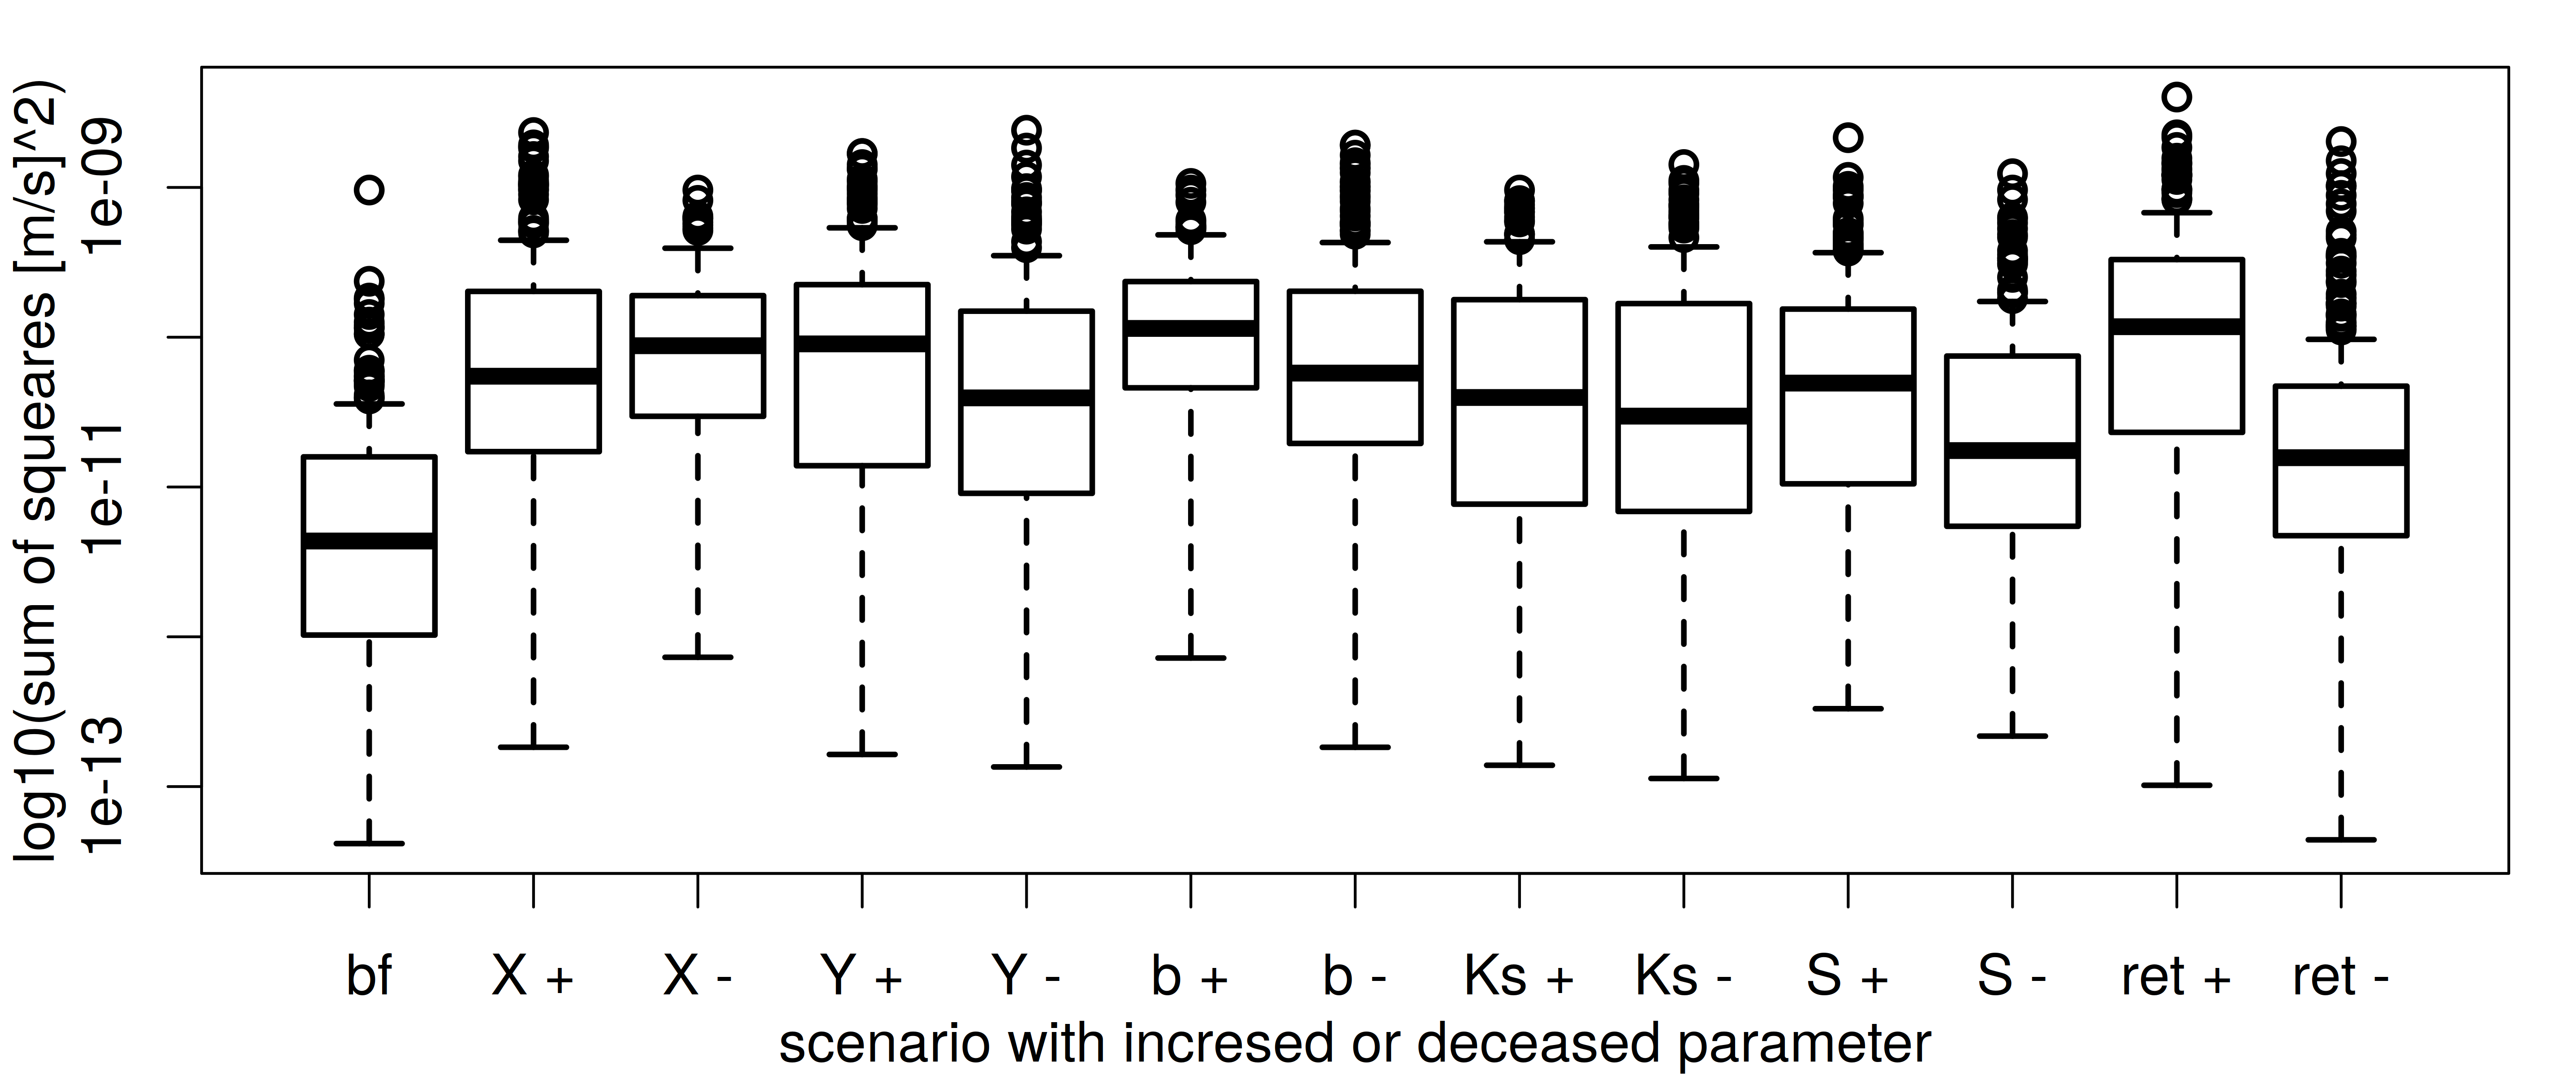
\includegraphics[width = \textwidth]{obr/sens.png}
        {\it Sensitivity of model parameters. bf - best fit: SS for all optimized model runs; parameter (+) and (-) stands for parameter increase based on factors in Tab. 1}
    \end{column}
\end{columns}
Functionalities of python package Scipy were used to perform optimization \citep{scipy}.
\end{block}

% 
\subsection{Model parameters and textural classes}
\begin{block}{Model parameters and textural classes}
\begin{columns}
    \begin{column}{0.2\textwidth}
            \begin{itemize}
                \item Infiltration parameters fitted with data
                \item Eq. \ref{eq:manning} parameters were optimized with differential evolution
                \item Effect of textural class and soil fraction to each parameter was tested
                \item Each experiment was optimized separately
            \end{itemize}
            {\it Parameter margins for optimization}
        \begin{table}[]
            \small
            \begin{tabular}{lllll}
            \hline
            \hline
            Parameter: & X & Z & b & ret \\
            \hline
            Max & 30 & 5 & 4 & 0 \\
            Min & 1 & 0.01 & 1 & -0.5 \\
            \hline
            \hline
            \end{tabular}
        \end{table}
        \vspace{1.5cm}
        \justifying
        {\it Example of model output during optimization}
        
        \centering
        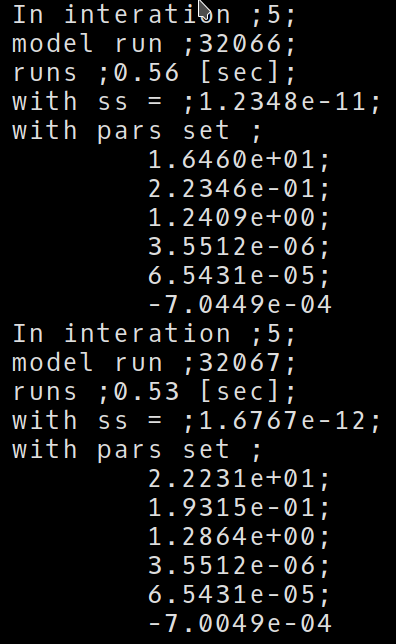
\includegraphics[width = 0.75\textwidth]{obr/cli.png}
    \end{column}
    \begin{column}{0.8\textwidth}
        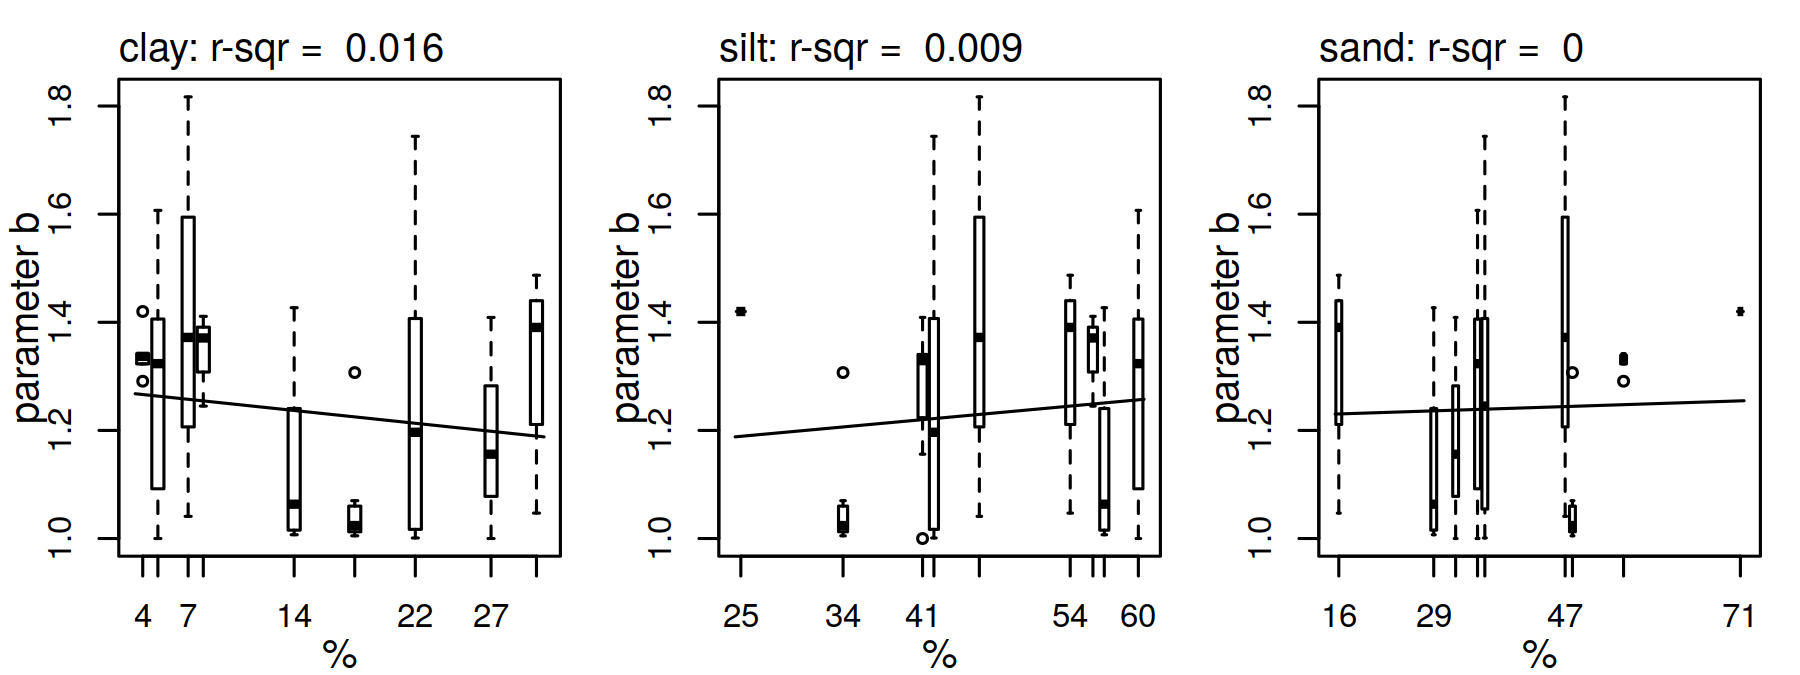
\includegraphics[width = \textwidth]{obr/bfittex.png}\\
        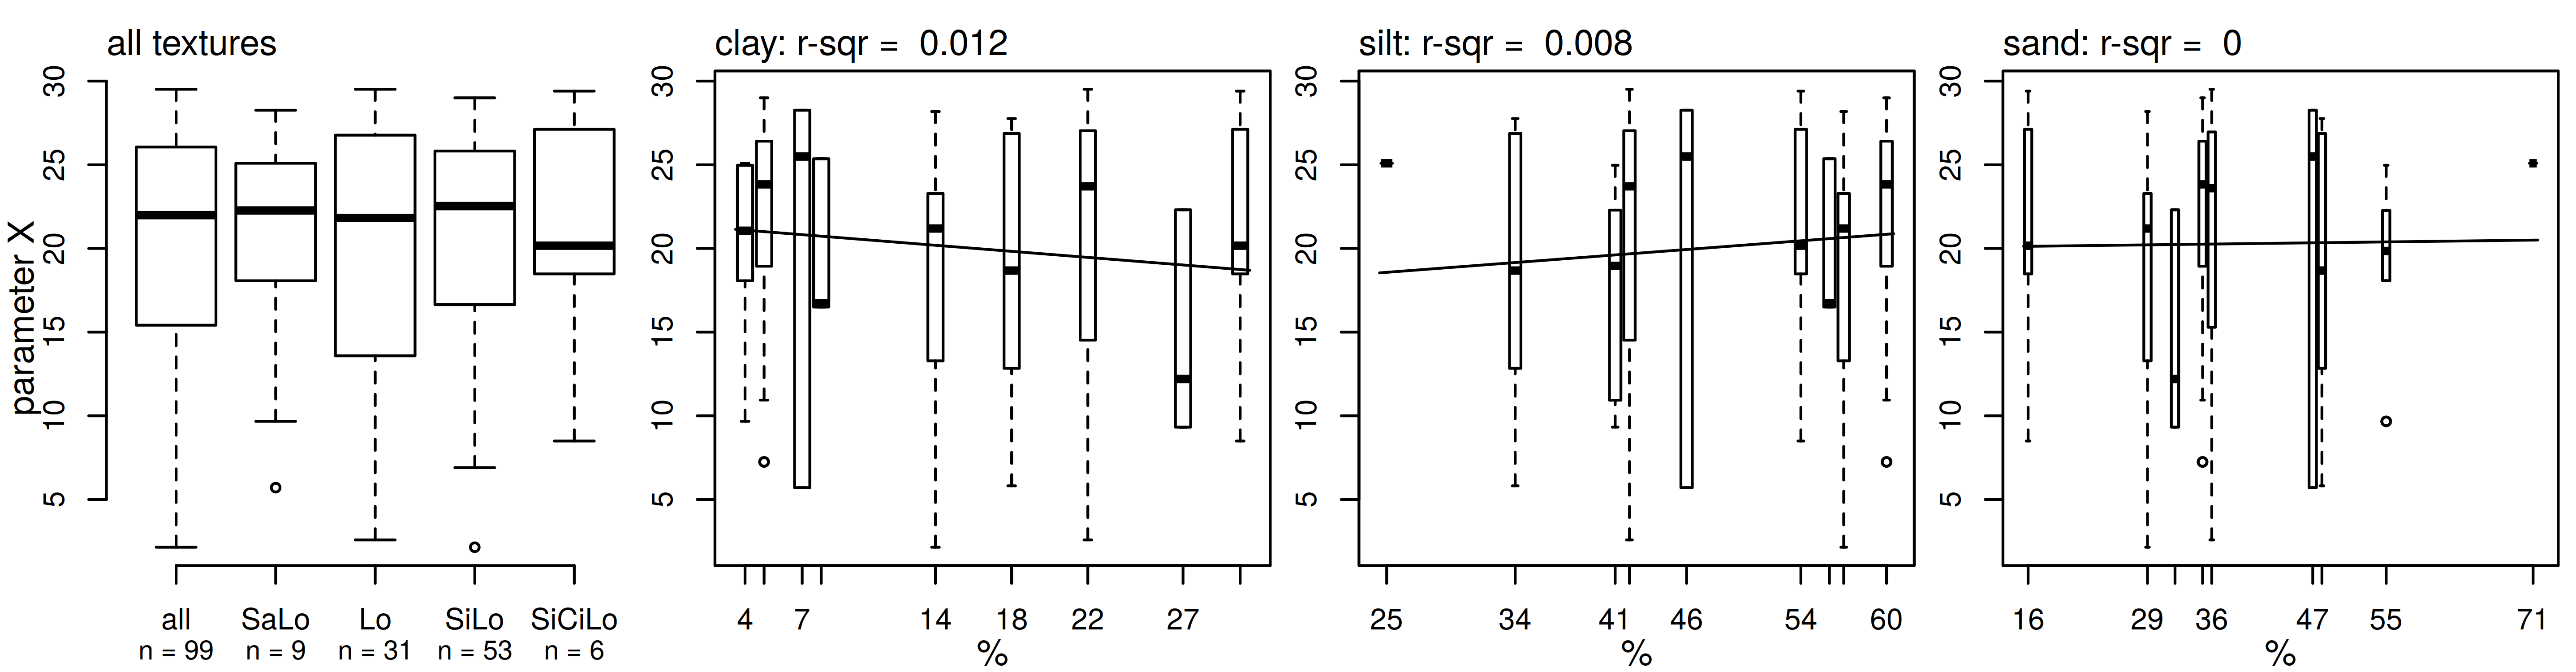
\includegraphics[width = \textwidth]{obr/Xfittex.png}\\
        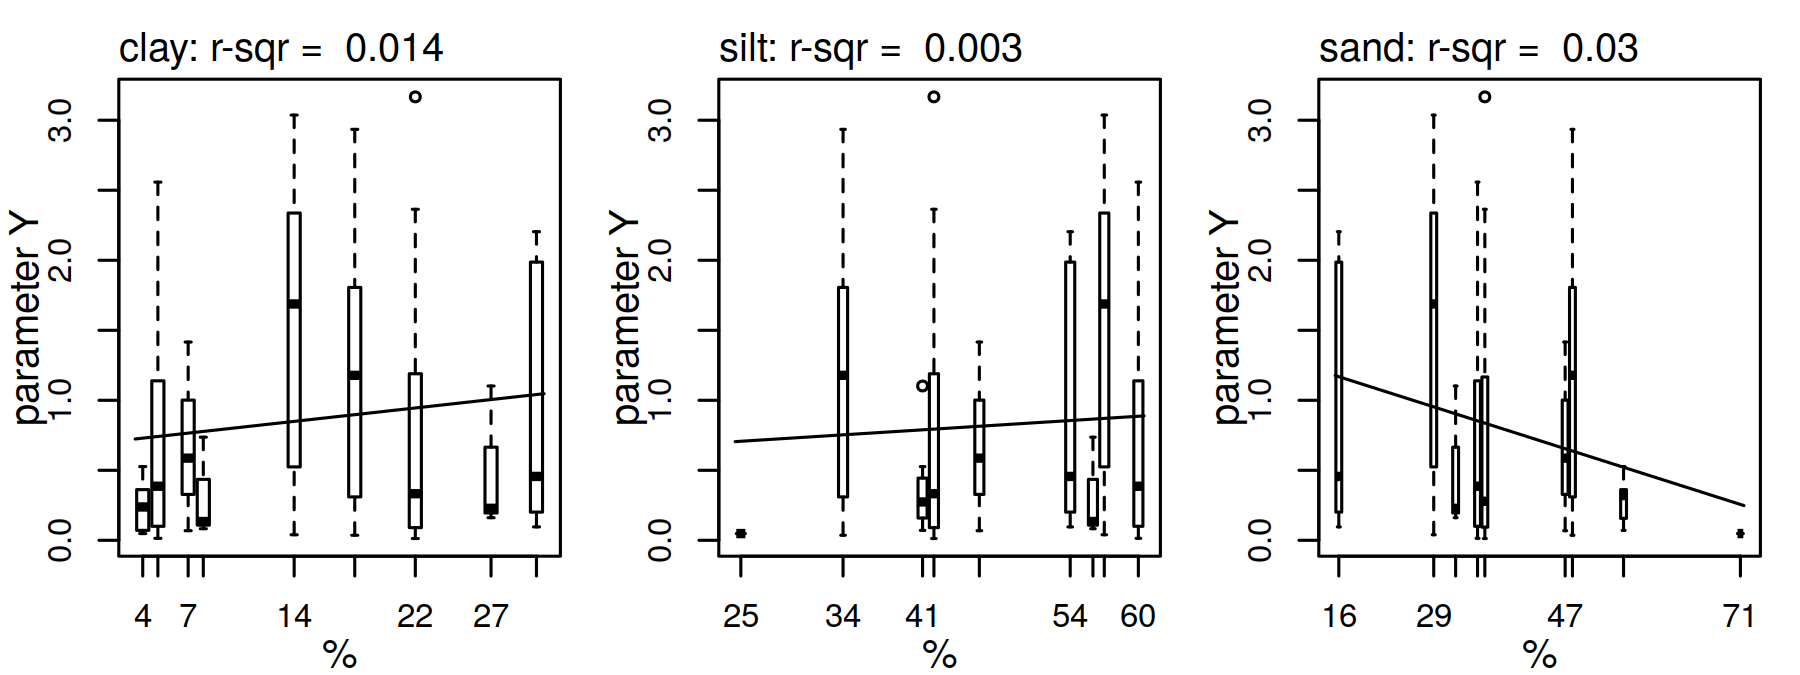
\includegraphics[width = \textwidth]{obr/Yfittex.png}
        {\it Figures shown optimized parameters. Top bar shown results of parameter b, middle bar shown results of parameter Y, and bottom bar shown results of parameter Y. Left graph shows values for textural class. Second to fourth graph shows parameter values for each soil fraction.}
    \end{column}
\end{columns} 

\end{block}

% 
\subsection{Uncertainty analyses: Monte Carlo runs}
\begin{block}{Uncertainty analyses: Monte Carlo runs}
\begin{columns}
    \begin{column}{0.25\textwidth}
        \begin{itemize}
            \item 10000 Monte Carlo simulations for each experiment
            \item Random sampling in the parameter space
            \item Nash Sutcliffe model efficiency (NS) for model run comparison
            \item NS greater than one accepted
            \item Among and inter textural class variation is displayed
        \end{itemize}
        GNU Parallel software was used during optimization and Monte Carlo simulations \citep{Tange2011a}. 
        \end{column}
        \begin{column}{0.75\textwidth}
            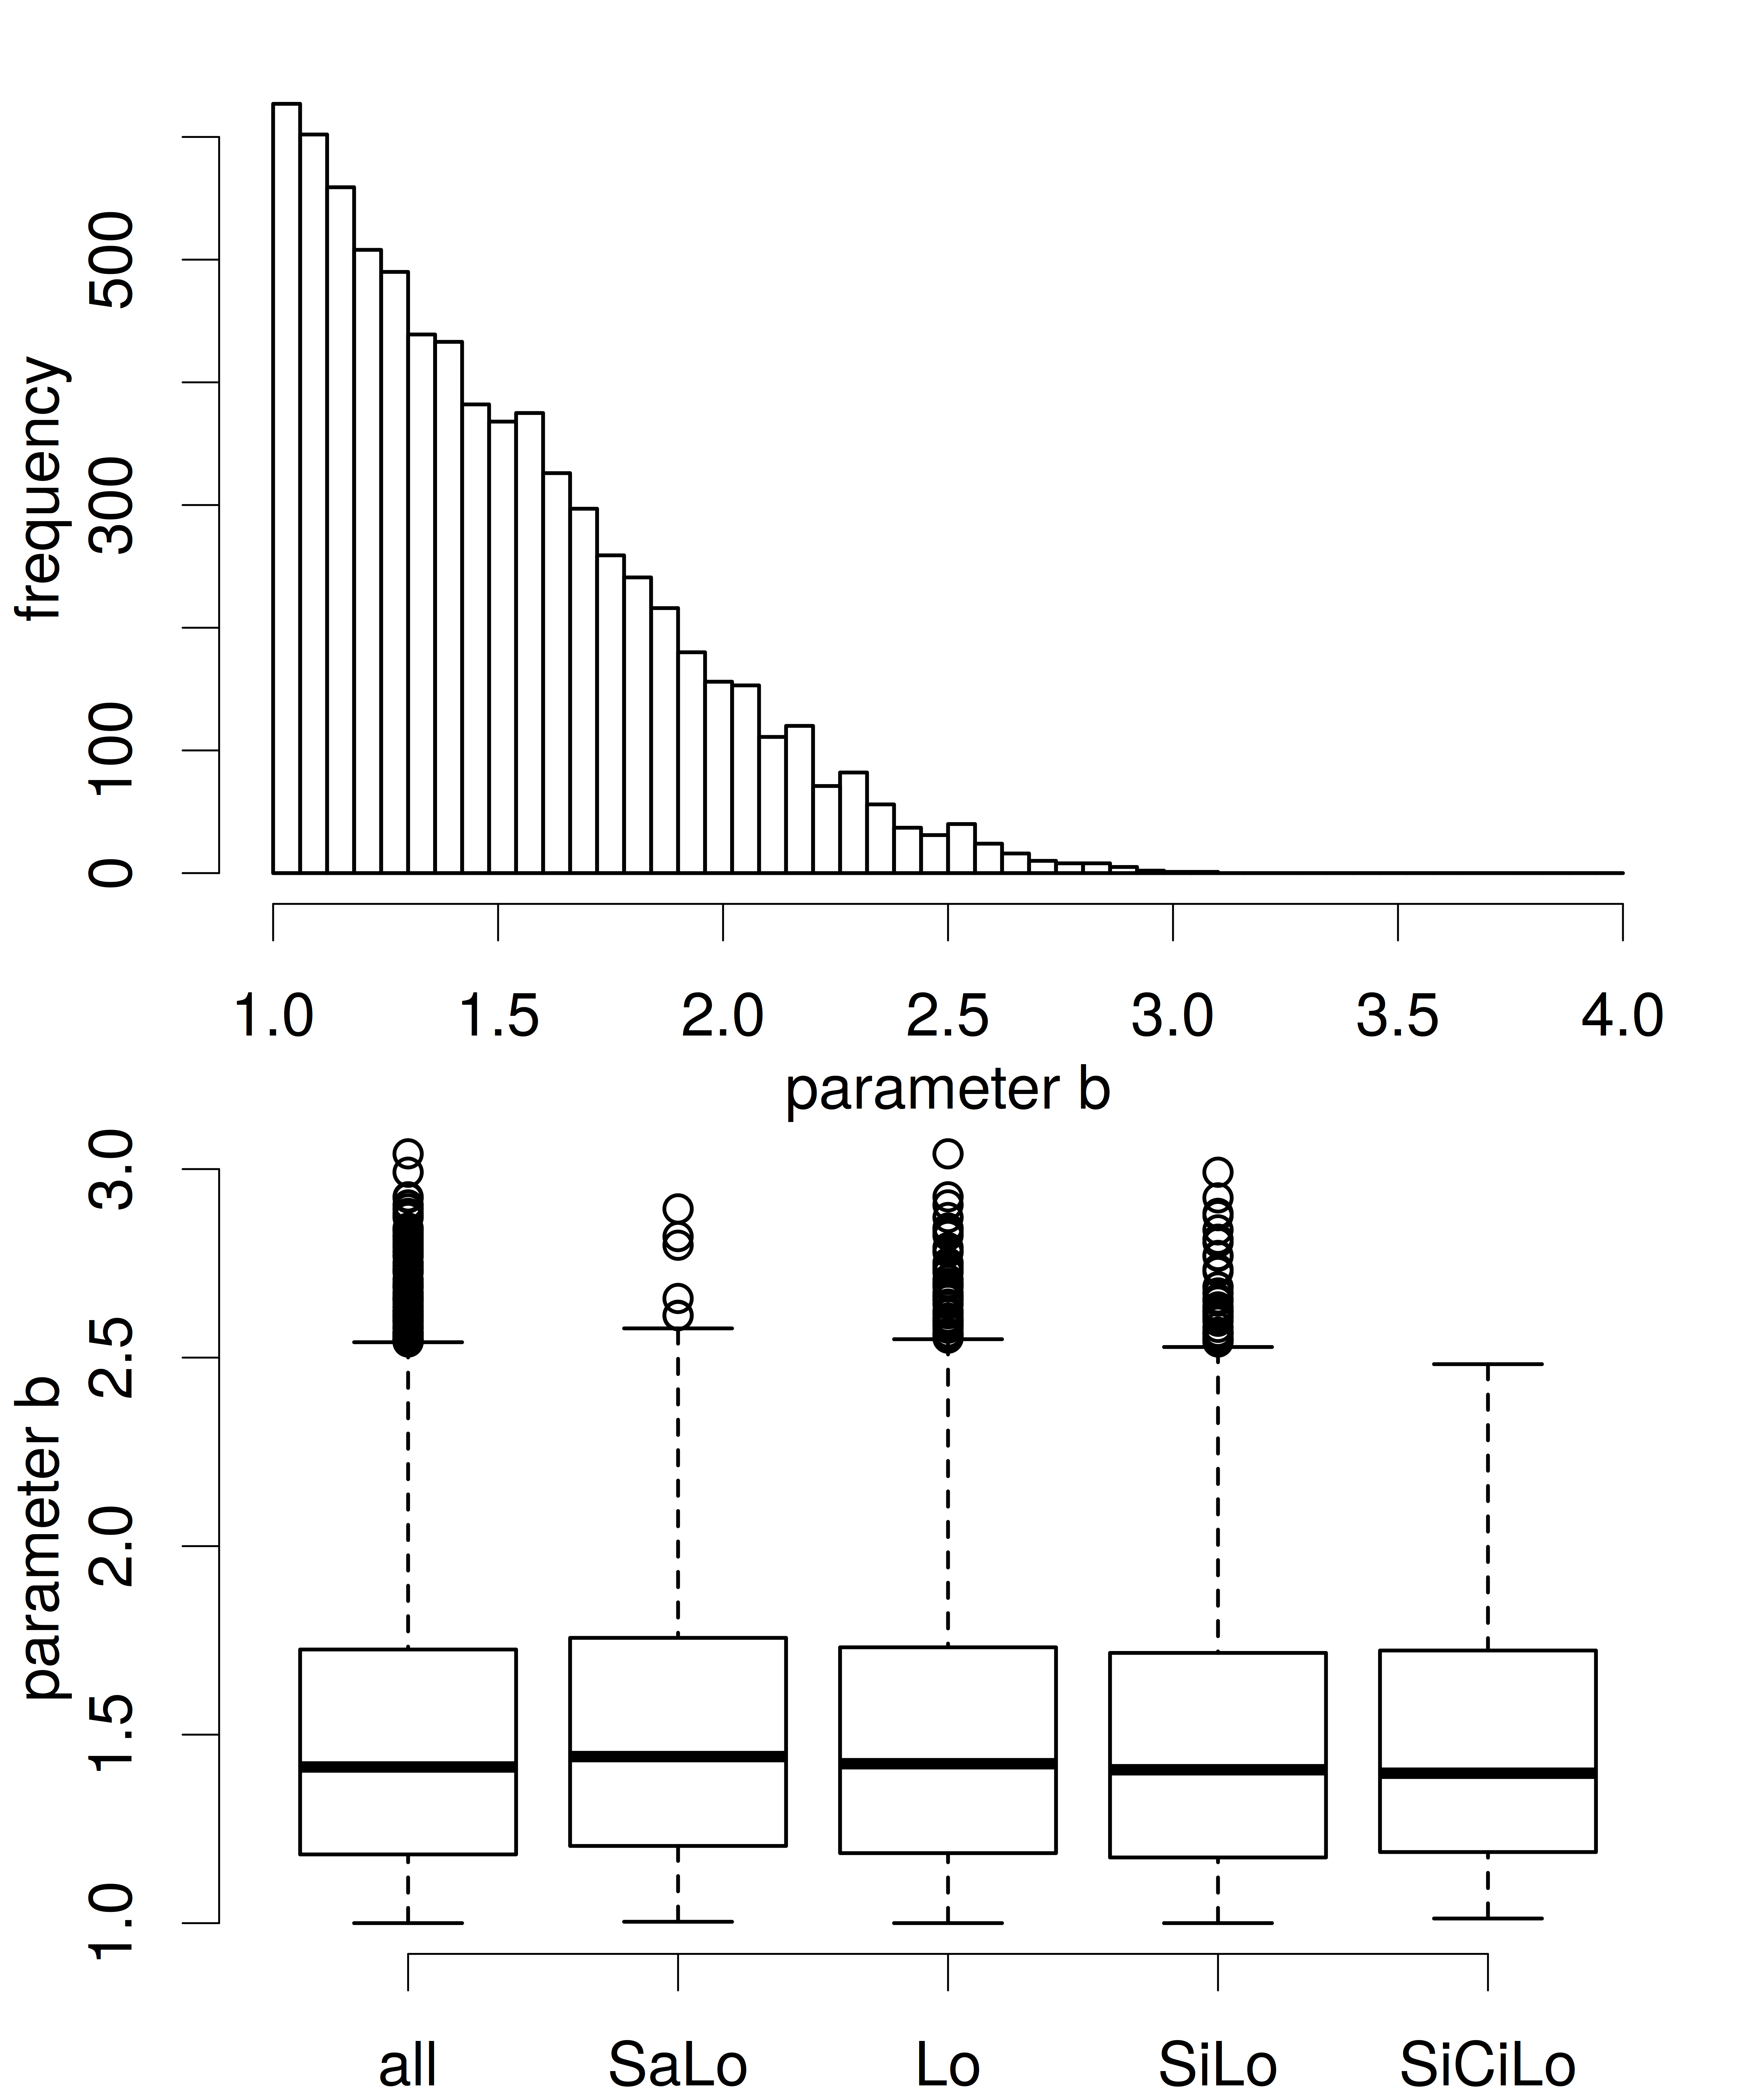
\includegraphics[width = 0.3\textwidth]{obr/mc_b.png}
            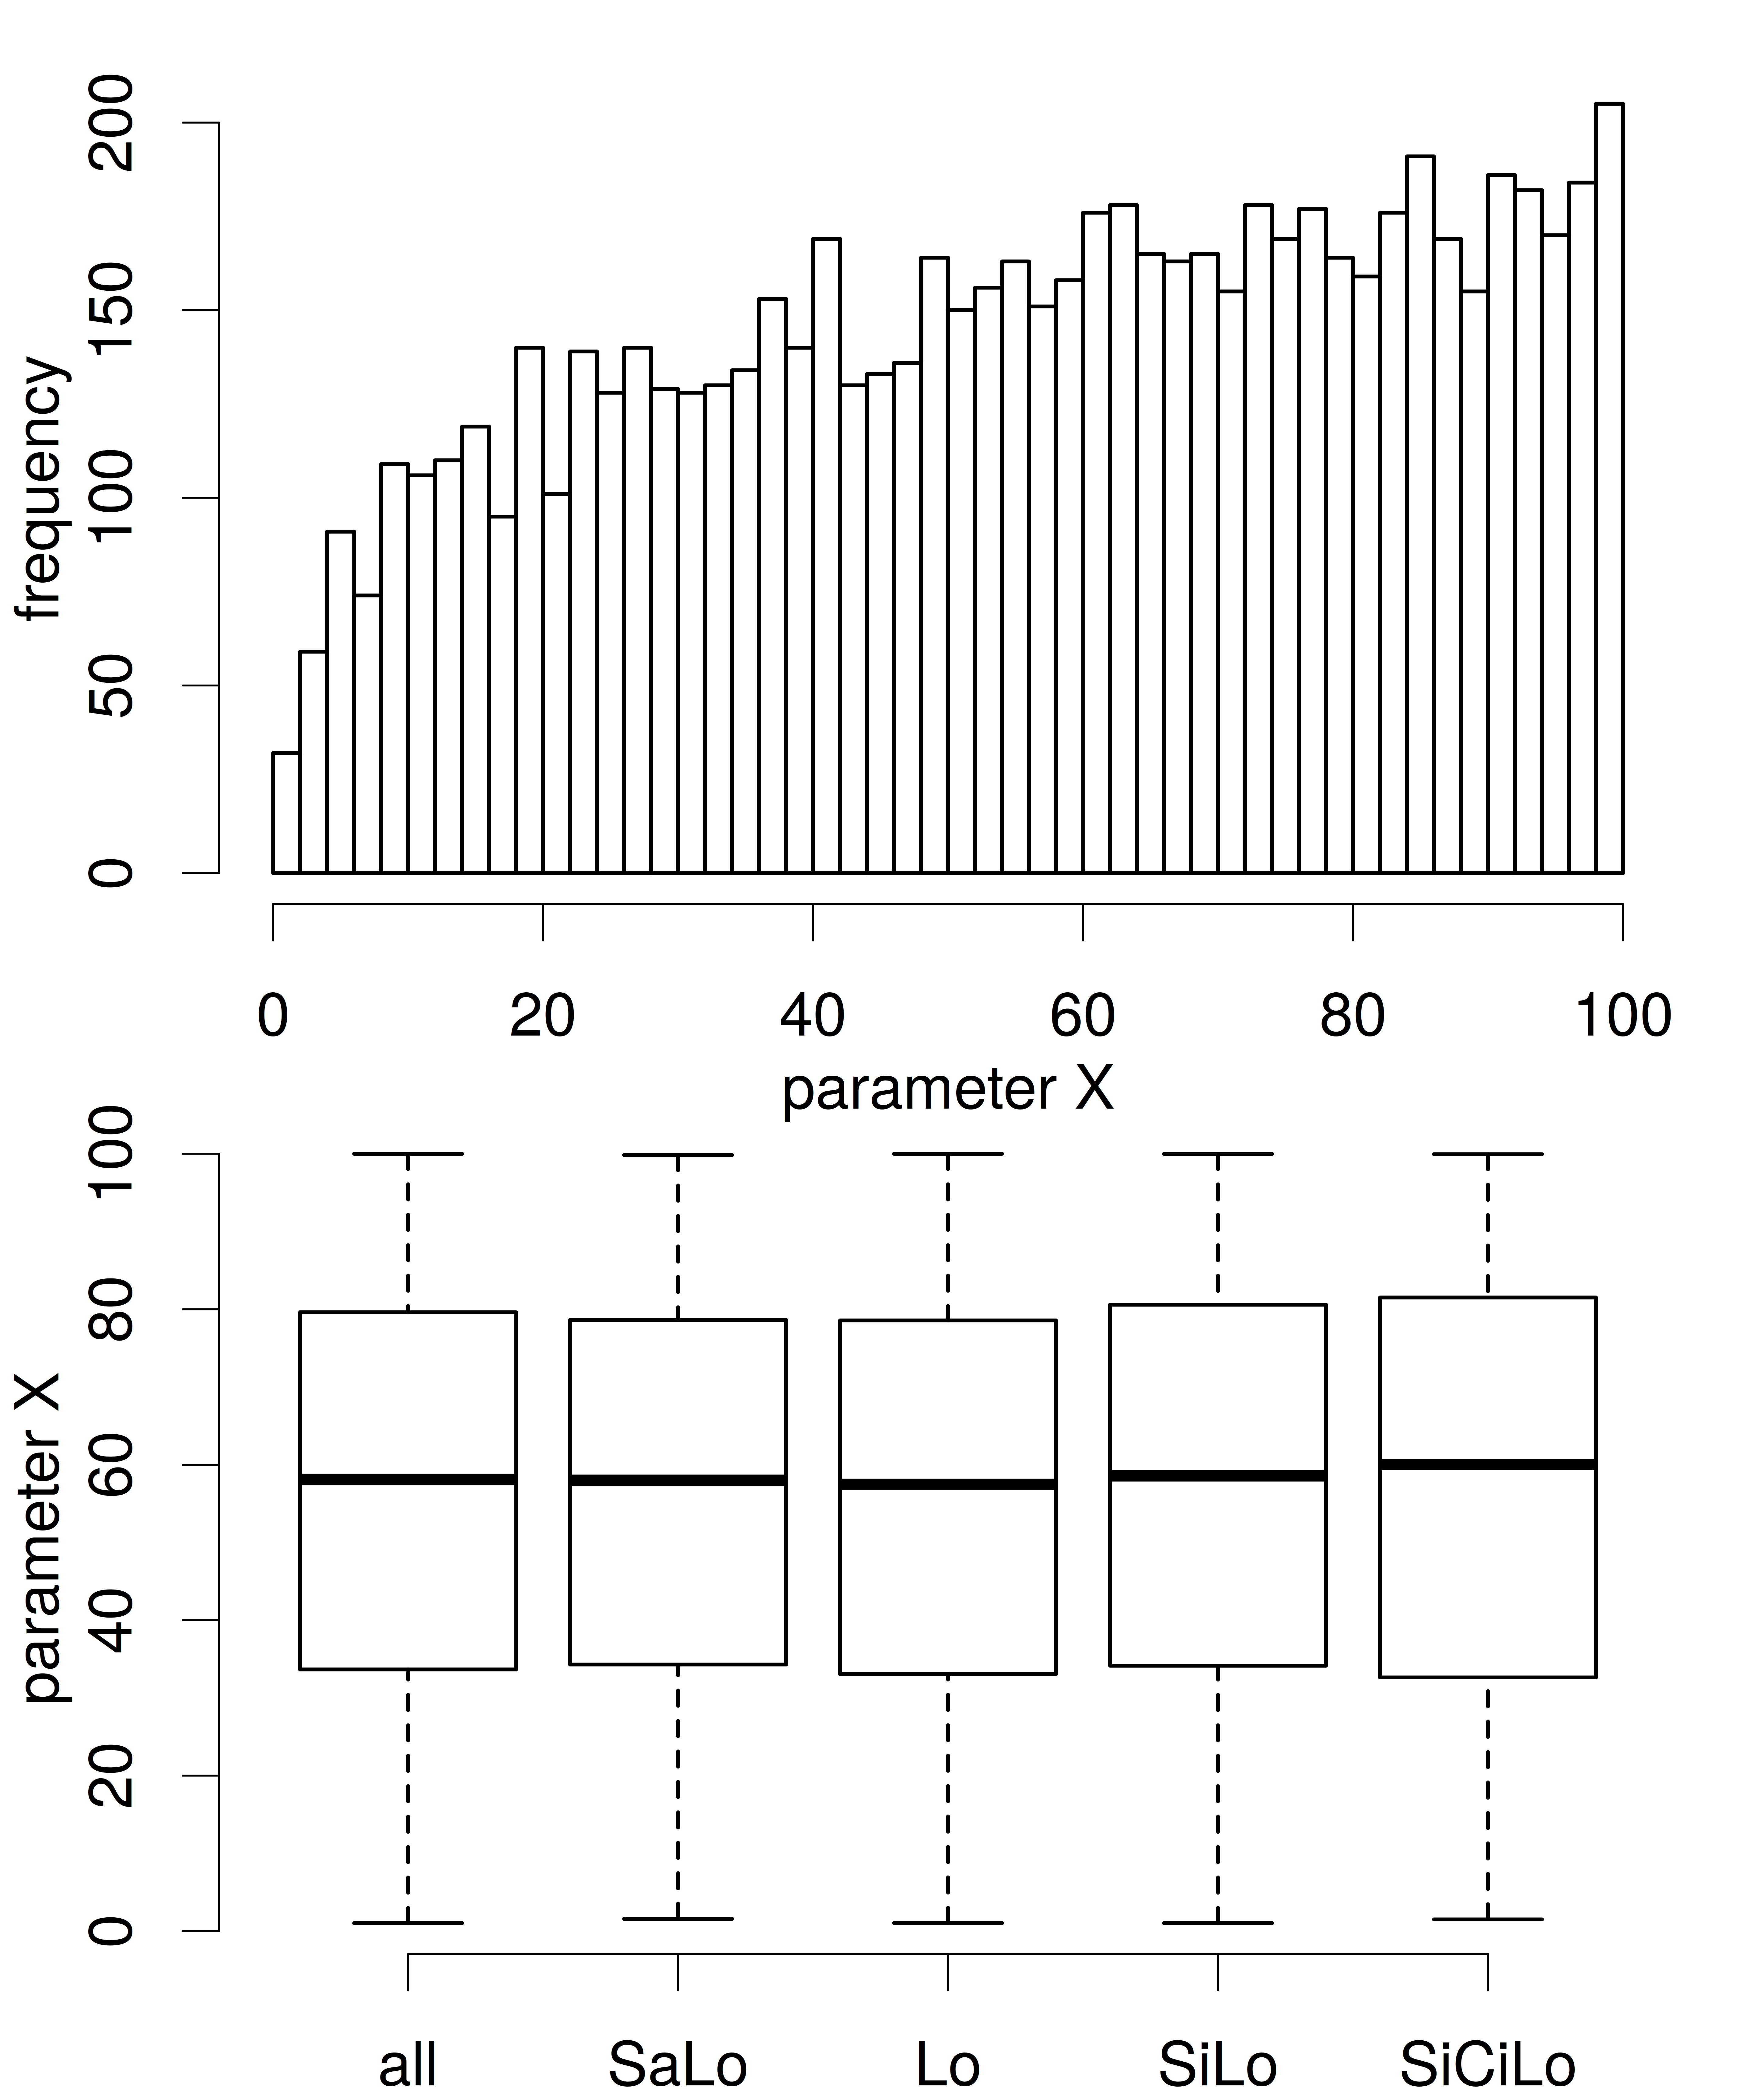
\includegraphics[width = 0.3\textwidth]{obr/mc_x.png}
            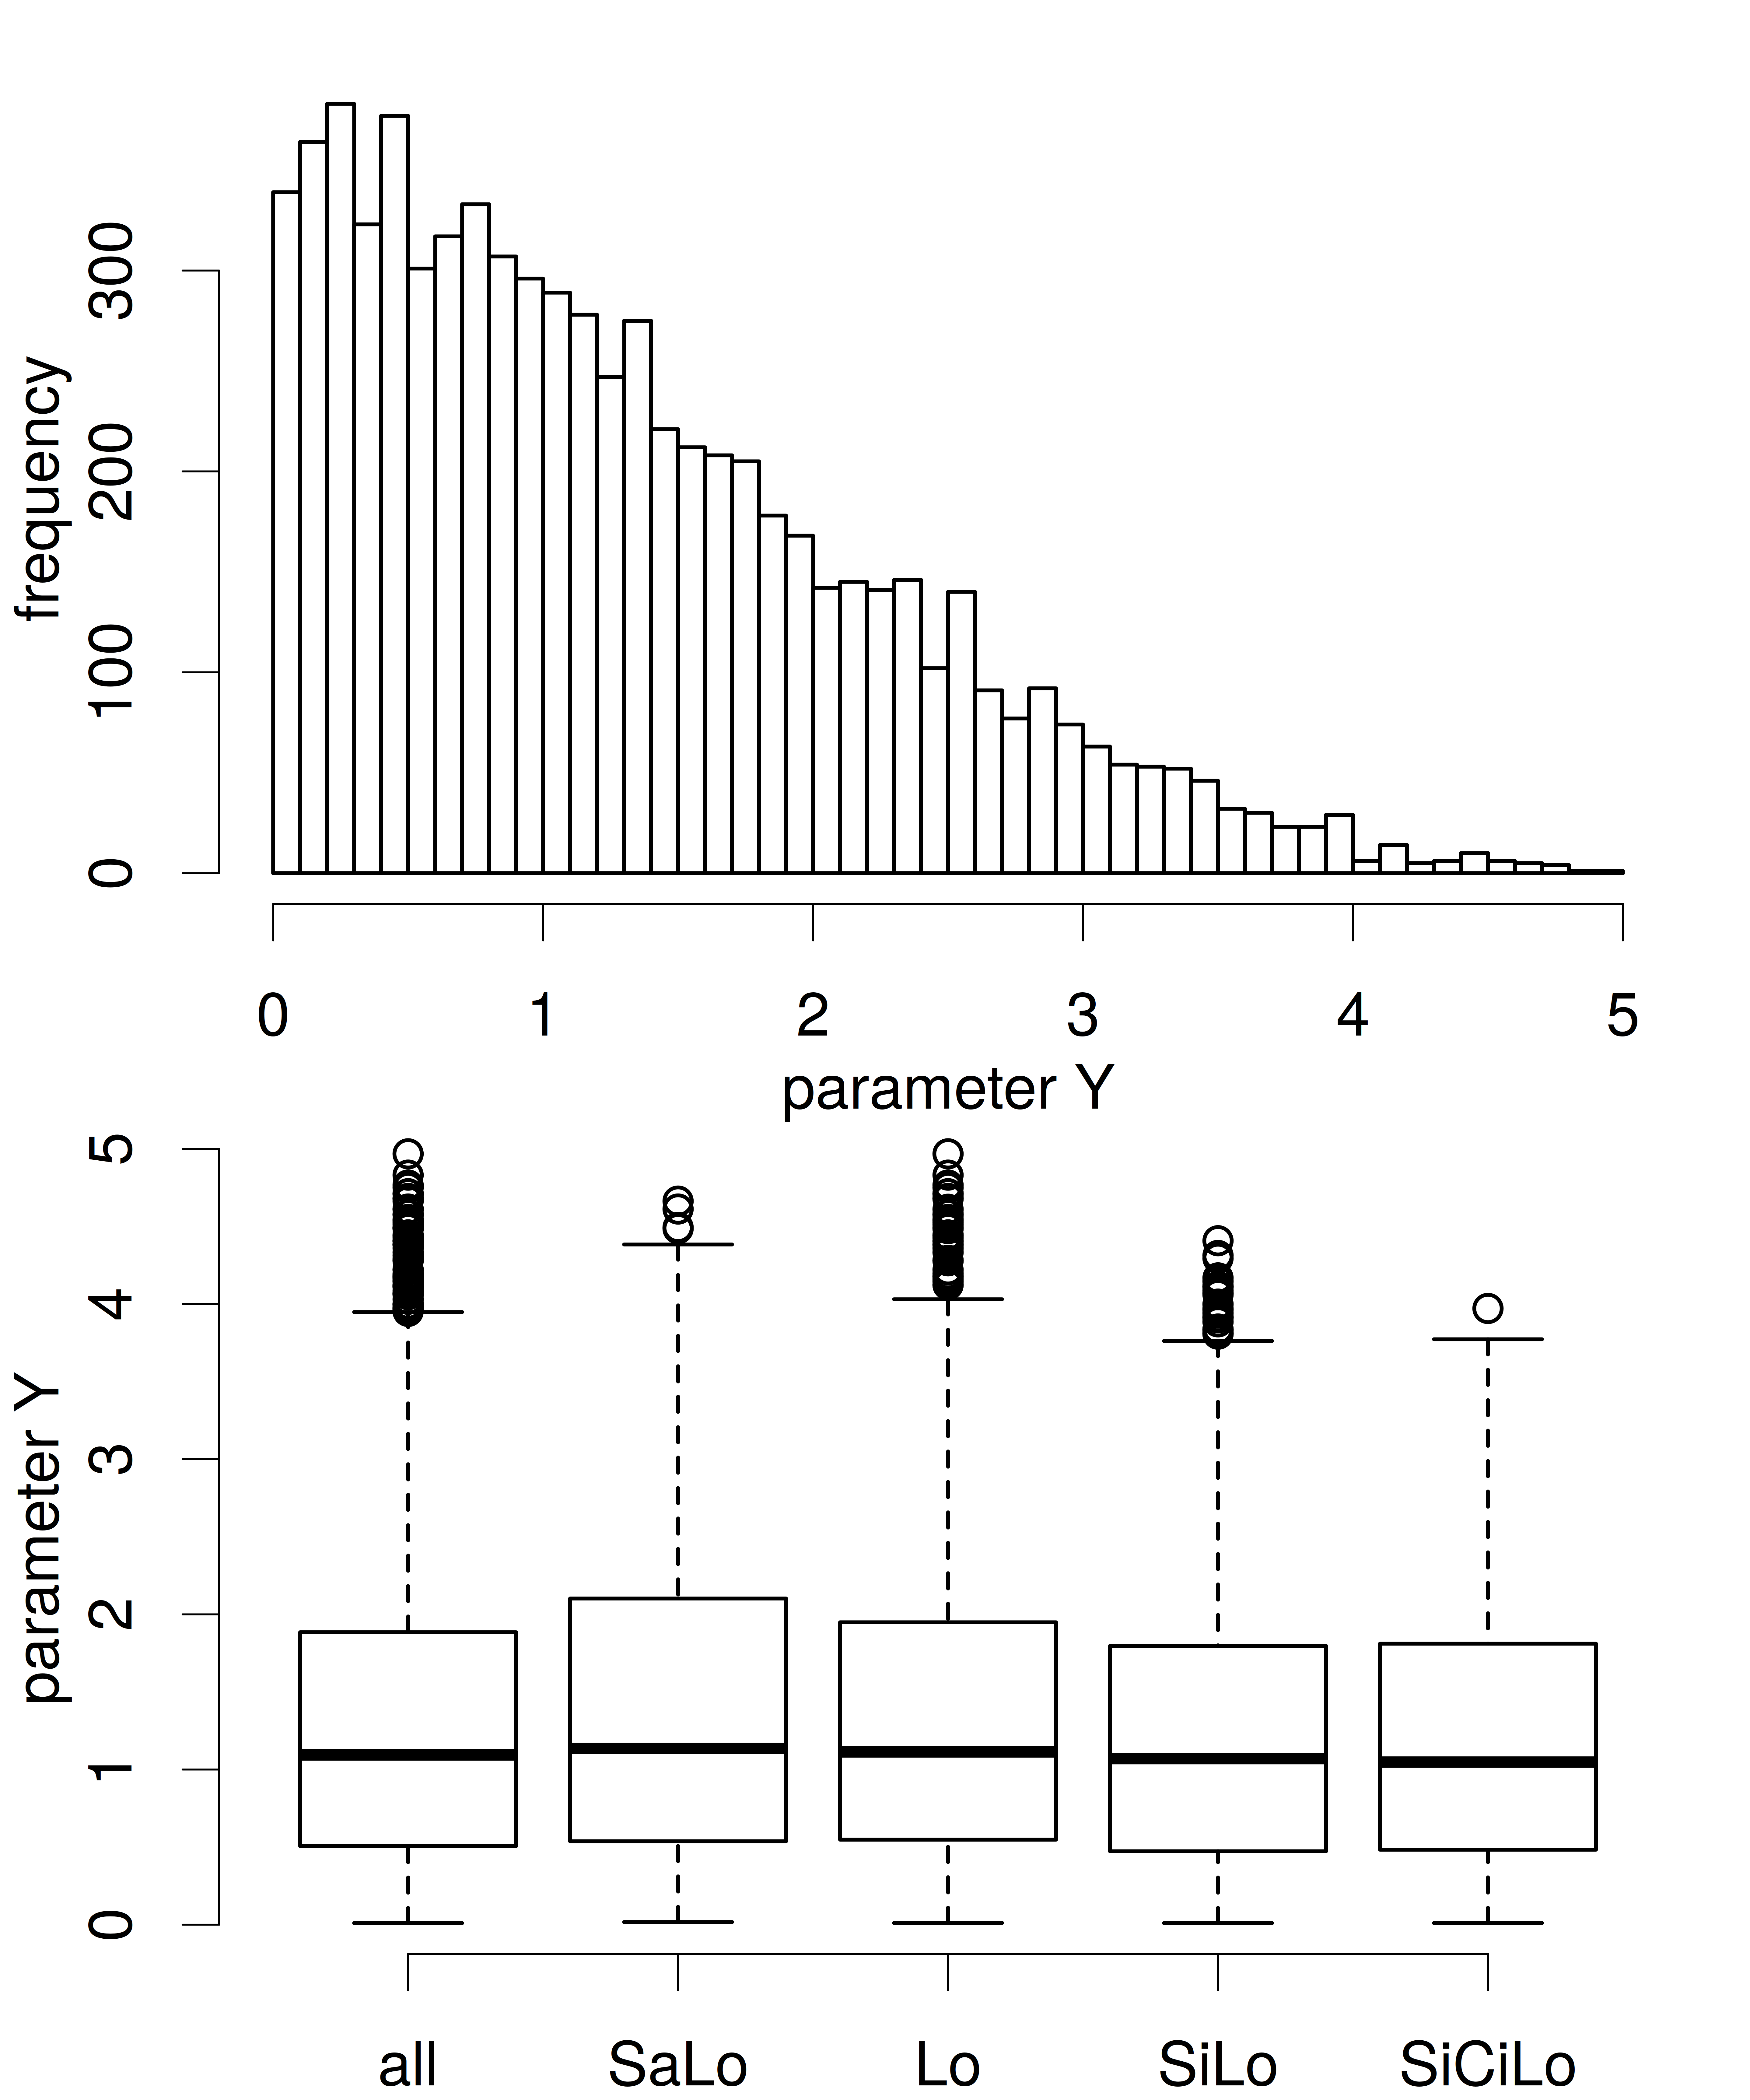
\includegraphics[width = 0.3\textwidth]{obr/mc_y.png}
            {\it  Histogram of excepted model runs for a given parameter (top); Box-plots for for all aggregated values and each soil textural class (bottom)}
        \end{column}
    \end{columns}
\end{block}















